\documentclass[border=6pt]{standalone}
\usepackage{tikz}
\usetikzlibrary{arrows.meta,backgrounds}

\begin{document}
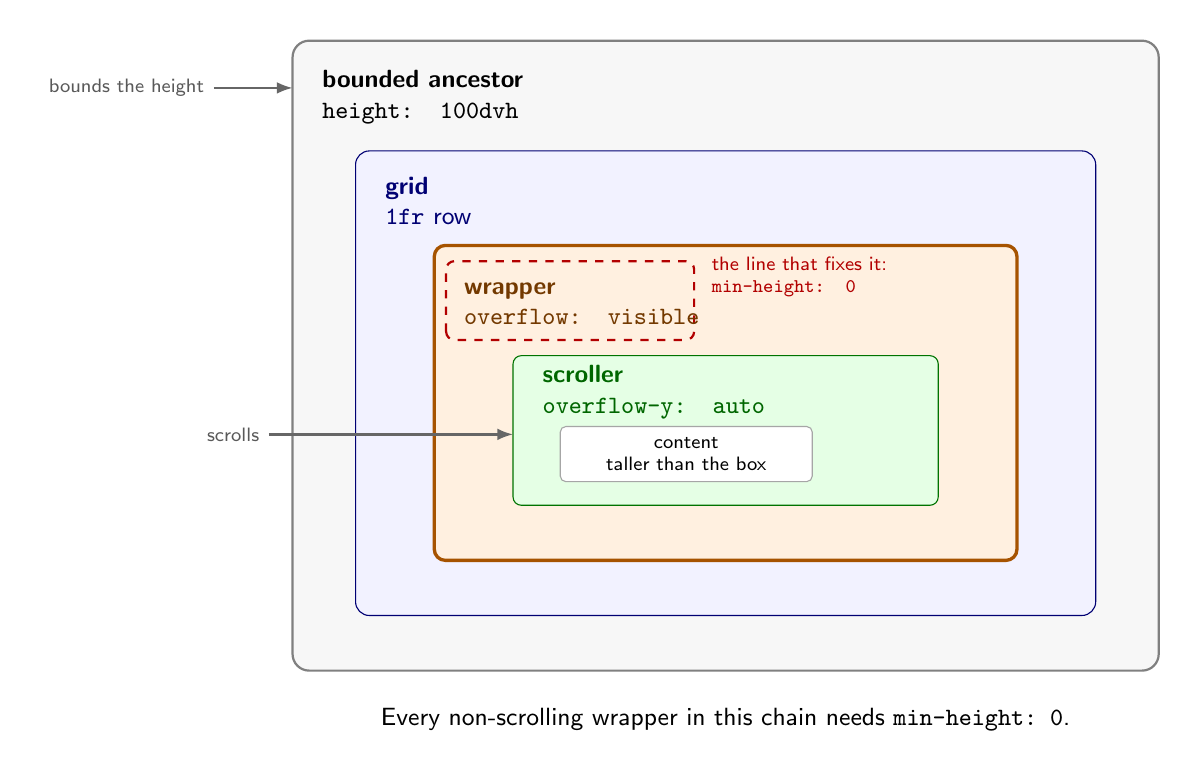
\begin{tikzpicture}[
  font=\sffamily\small,
  show background rectangle,
  background rectangle/.style={fill=white},
  arrow/.style={-{Latex[length=2mm]}, thick, draw=black!60},
  annot/.style={font=\sffamily\scriptsize, text=black!65, align=right, anchor=east},
  label/.style={anchor=north west, align=left, inner sep=2pt}
]
  % rectangles
  \draw[rounded corners=6pt, fill=gray!6, draw=black!50, thick]
    (0,0) rectangle (11,8);

  \draw[rounded corners=5pt, fill=blue!5, draw=blue!45!black]
    (0.8,0.7) rectangle (10.2,6.6);

  \draw[rounded corners=4pt, fill=orange!12, draw=orange!65!black, very thick]
    (1.8,1.4) rectangle (9.2,5.4);

  \draw[rounded corners=3pt, fill=green!10, draw=green!45!black]
    (2.8,2.1) rectangle (8.2,4.0);

  \draw[rounded corners=2pt, fill=white, draw=black!35]
    (3.4,2.4) rectangle (6.6,3.1);

  \draw[red!70!black, dashed, thick, rounded corners=3pt]
    (1.95,4.2) rectangle (5.1,5.2);

  % labels
  \node[label] at (0.3,7.7)
    {\textbf{bounded ancestor}\\\texttt{height: 100dvh}};

  \node[label, text=blue!45!black] at (1.1,6.35)
    {\textbf{grid}\\\texttt{1fr} row};

  \node[label, text=orange!45!black] at (2.1,5.0)
    {\textbf{wrapper}\\\texttt{overflow: visible}};

  \node[label, text=green!40!black] at (3.1,3.95)
    {\textbf{scroller}\\\texttt{overflow-y: auto}};

  \node[font=\sffamily\scriptsize, align=center] at (5.0,2.75)
    {content\\taller than the box};

  \node[anchor=west, text=red!70!black, font=\sffamily\scriptsize, align=left]
    at (5.2,5.0) {the line that fixes it:\\\texttt{min-height: 0}};

  % annotations
  \node[annot] (a1) at (-1.0,7.4) {bounds the height};
  \draw[arrow] (a1) -- (0,7.4);

  \node[annot] (a3) at (-0.3,3.0) {scrolls};
  \draw[arrow] (a3) -- (2.8,3.0);

  % bottom note
  \node[anchor=north, align=center, text width=10.5cm, font=\sffamily\small]
    at (5.5,-0.35) {Every non-scrolling wrapper in this chain needs \texttt{min-height: 0}.};
\end{tikzpicture}
\end{document}
